\subsection{Disponibilidad vs Accesibilidad.}
    
Como mencionamos en la introduccion de este capitulo, los datos pueden estar disponibles en la fuente original, pero no por
ello significa que estos sean accesibles.
Los retos a los que nos encontramos con los datos crudos, directos de la fuente de origen, son los siguientes:
    
    \begin{itemize}
        \item \textbf{Localizacion}. Los datos se encuentran disponibles en portales de datos abiertos organizados 
        y estructurados, normalmente se necesita una tarea de busqueda y seleccion
        a veces complicada. Aunque las empresas ponen cada vez mas de su parte en ofrecer una interfaz 
        agradable y funcional a los usuarios, esta tarea requiere de un trabajo de investigacion por parte del usuario,
        ya que posiblemente, debera buscar en distintos portales.
        \item \textbf{Extraccion}. Los datos suelen estan disponibles a traves de una interfaz de programacion 
        de aplicaciones (API) no facilmente interpretable por el usuario medio. Normalmente cuenta con 
        un documento que describe cada uno de los campos y valores que se presentan en el documento y como utilizar la API.
        \item \textbf{Interpretabilidad}. Usualmente los datos estan representados en un formato para ser procesado por 
        algun software, por lo que su lectura resulta complicada por el usuario medio, en el mejor de los casos, 
        estaran representados en una tabla y aun asi, sera muy dificil de extraer informacion.
        \item \textbf{Infraestructura}. Por ejemplo, el almacenamiento. Los datos publicados son los mas recientes, por lo que no hay manera de obtener 
        un historico de los datos si no son almacenados periodicamente. Una vez extraidos los datos, el usuario debera 
        contar con una infraestructura que le permita almacenar los datos.
        \item \textbf{Automatizacion}. Este proceso tiende a ser arduo, por lo que sera necesario automatizarlo, de otra 
        forma el esfuerzo requerido por el usuario para extraer la informacion no le compensara. 
        \item \textbf{Awarenes}. El usuario necesitara saber que tiene este recurso y puede utilizarlo.
         
    \end{itemize}
    
Por lo tanto, no podemos decir que estos datos sean accesibles de una forma util para el usuario medio.\\
\subsubsection{How to solve it.} 

Deberemos proporcionar la informacion requerida por el usuario de forma directa, facil de leer e interpretar. Ademas proporcionaremos
la infraestructura necesaria para que el usuario solo tenga que consultar los datos y automatizaremos los procesos que deban repetirse
periodicamente.
 
\subsubsection{How we solve it. Aire Guru.} 

Nuestra herramienta utiliza los datos de calidad del aire proporcionados por el ayuntamiento de Malaga en su portal de datos abiertos.\footnote{\url{https://datosabiertos.malaga.eu/}}\\
\begin{figure}[h]
    \centering
   \subfigure[Pagina principal]
    {\includegraphics[width=5.5cm  ]{OpenDataPortal}}
    \hfill
    \subfigure [Categoria medio ambiente]
       { 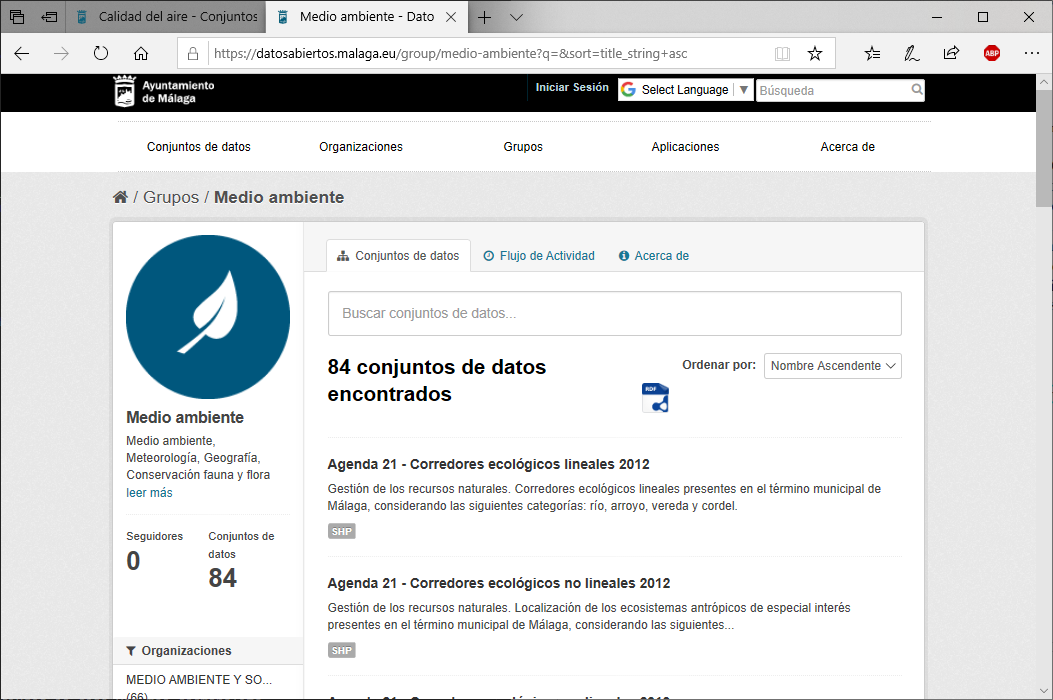
\includegraphics[width=5.5cm]{openDataPortalEnviromentCategory}}
    \vfill
     \subfigure[GeoJson Document]
     { \centering 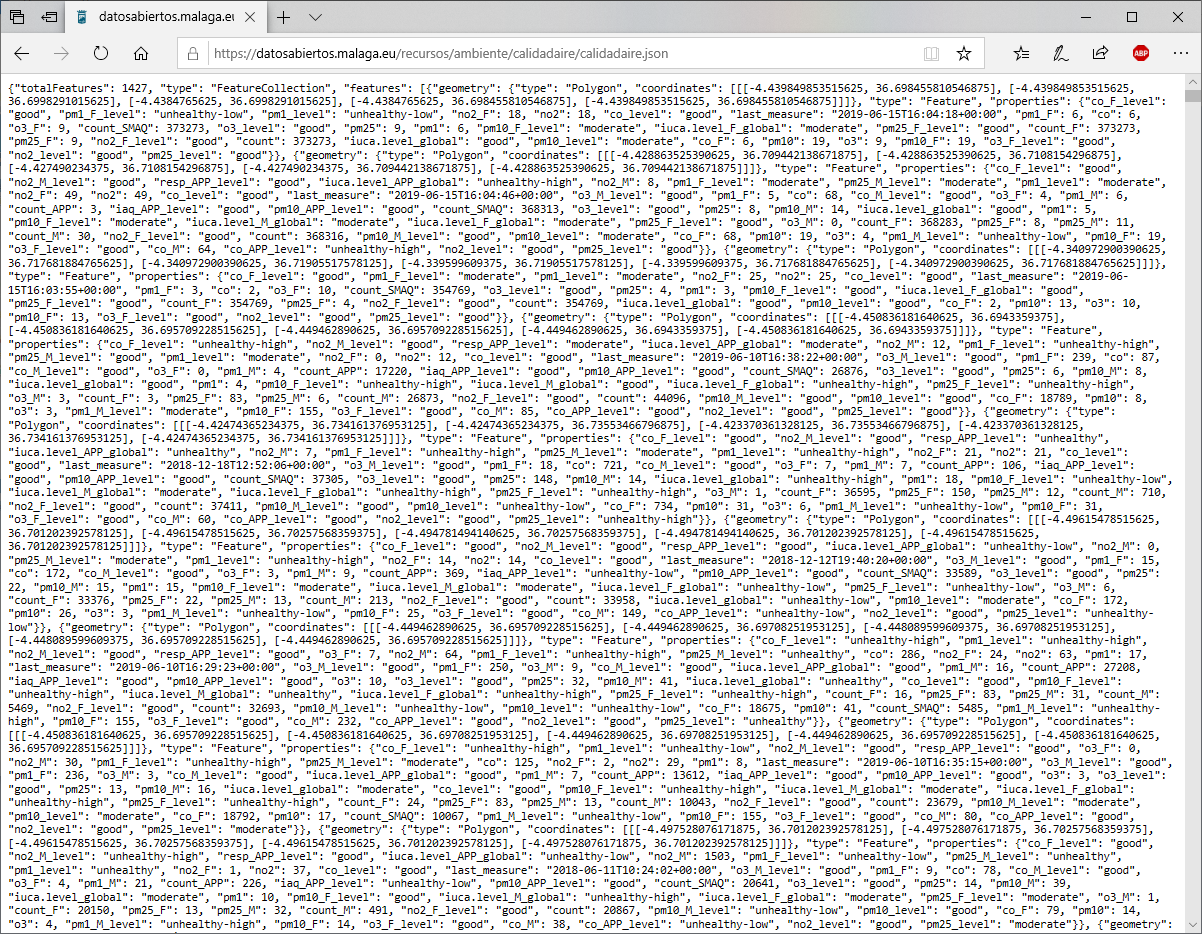
\includegraphics[width=4.75cm]{geoJsonAirQualityDataRaw}}
  
  \caption{Open Data Portal Malaga}
    \end{figure}

    Este portal de datos ofrece una oferta de categorias representados por iconos, por lo que es necesario saber en que categoria se clasifica el conjunto
de datos, una vez que se accede a la categoria, tenemos una barra buscadora que nos permite insertar las palabras claves para buscar el conjunto de datos
deseado.\\

En este caso puede pulsarse sobre el enlace y este abrira los datos en una nueva pestana, por lo que la utilizacion de un sistema informatico
para la descarga de los datos no es extrictamente necesario, pero podemos ver que ver que el formato no es legible, al menos desde el punto
de vista humano. 
Se actualiza cada hora, por lo que si queremos acceder a unos datos en concreto, deberemos repetir la operacion periodicamente.
Un valor importante de este conjunto de datos es saber la evolucion de la polucion por zonas, la extraccion de esta informacion no es posible
si no se realiza un almacenado de los datos.

Aire Guru automatiza el proceso de recoleccion de los datos mediante un trabajo CRON que ejecuta un script implementado en JavaScript periodicamente. Este lee 
los datos de la url, los procesa, limpia y almacena en una base de datos MongoDB.

\begin{figure}[ht]
    \centering
    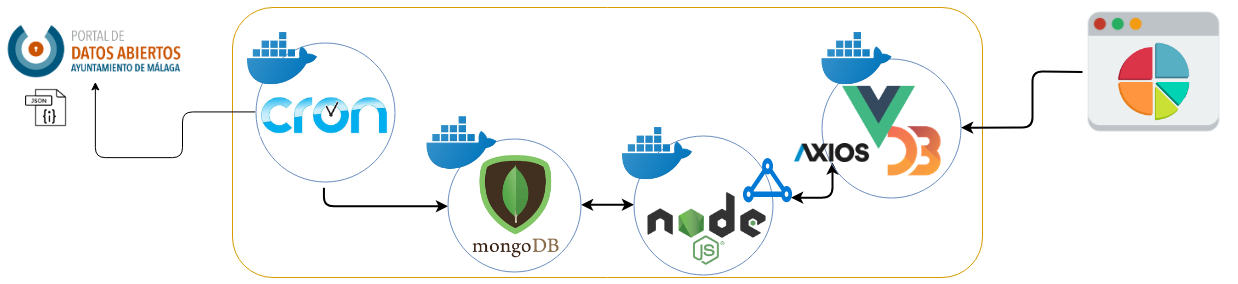
\includegraphics[width=12cm]{aireGuruArquitecture}
    \caption{Arquitecture Aire Guru}
\end{figure}

Mediante una interfaz web, muestra los datos al usuarios.

\begin{figure}[ht]
    \centering
    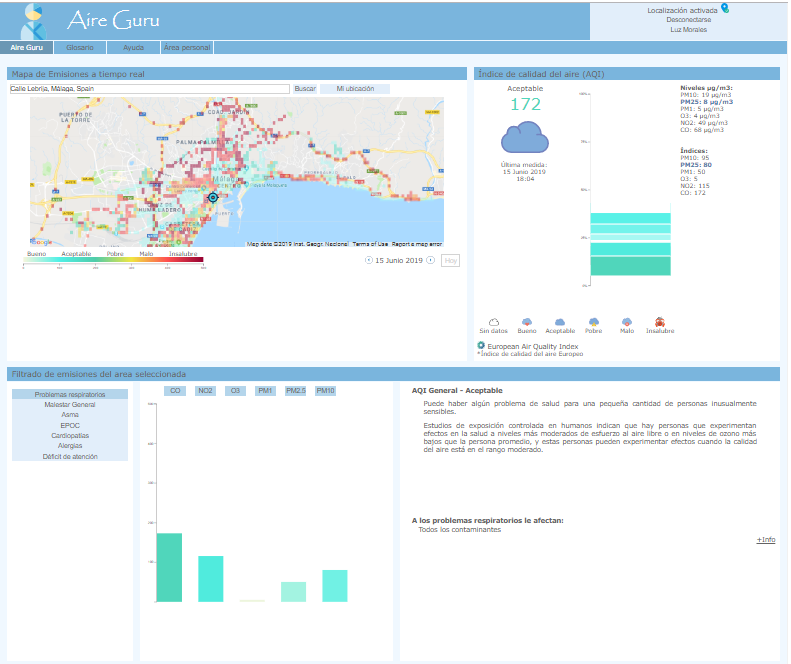
\includegraphics[width=9cm]{aireGuru}
    \caption{Aire Guru. Web Interface}
\end{figure}

Actualmente se trabaja en dar a conocer este producto. De momento esta disponible en el portal de datos abiertos en la pestana de aplicaciones.
.\footnote{\url{https://datosabiertos.malaga.eu/aplicaciones}}\\


\paragraph{Evaluation} \mbox{}

\begin{itemize}
    \done Localizacion. La localizacion de los datos es directa, ya que ofrece informacion desde el primer momento en que se accede a la web. En la pagina principal
presenta los niveles de polucion en todas las zonas sin necesidad de realizar ninguna seleccion.
\done Extraccion. No es necesario ningun software o conocimientos informaticos para acceder la informacion.
\done Interpretabildad. Contine un mapa donde los niveles de polucion se presentan por colores. Estos colores estan definidos por una leyenda justo
debajo del mapa. Cuenta con un glosario donde se explica los conceptos expuesto en la pagina web, el significado de cada seccion y como
navegar por la pagina web.
\done Infraestructura. Implementa toda la arquitectura necesaria tanto de almacenaje, procesado como visualizacion.
\done Automatiza los procesos de recoleccion de datos y los calculos necesarios para mostrar la informacion al usuario. Por ejemplo, una pregunta simple 
seria saber a que nivel de polucion estamos rodeados en las coordenadas en la que nos encontramos. Con la informacion en crudo obtenida desde el portal, 
nos es una tarea imposible, pero si ardua si no contamos con un sistema que procese los datos. Aire Guru resulve este problema.
\crossed Awarenes. Deberia trabajarse en la publicidad de la plataforma y darla a conocer.
\end{itemize}
\newpage

 


